% !TeX spellcheck = en_US
% !TeX root = ../MS_analysis_thesis.tex
\section{Possibly Relevant Biomarkers} \label{section:relevant biomarkers}
In this section, we will discuss several biomarkers that will (or can) be used in the prediction of day quality for MS patients.

\subsection{Resting Heart Rate} \label{section:Resting Heart Rate}
Resting heart rate is defined as the heart rate of a person that has not been subjected to any form of stimulation or exertion.
For adults, the resting heart rate lies between 60 and 100 beats per minute.
However, this also depends on the fitness of the person.
Despite this variety, several studies have shown that a high heart rate is related with several risks \cite{cunha1997association}.
Therefore it seems desirable to have a low resting heart rate.
A lot of studies have addressed the importance of heart rate in healthy humans \cite{reunanen2000heart, benetos1999influence, fujiura2001heart}.
The resting heart rate can also be an interesting indicator for the prediction of day quality of MS patients.
However, there is hardly any literature about the classification of heart rate in rest from heart rate data.
Can we come up with an algorithm to extract this information?

Currently, the technology of photoplethysmography (PPG) is being used to develop small devices that can measure the heart rate \cite{tamura2014wearable}. 
This technology uses changes in blood volume in the tissue to determine the heart rate. 
The sensor contains a light source and a light detector.
The light is emitted through the skin using the light source and the reflected light is measured using the light detector. 
Because blood is red, it reflects red and absorbs green light. 
By using a green light source, the change in the light intensity is therefore related to the blood perfusion of the tissue and can provide information on the pulse rate.
When your heart beats, the blood flow in your wrist is greater, and so is the green light absorption. 
Between beats, the light absorption is less. 
By flashing the light many times per second, the number of heart beats per minute can be calculated.
%
\begin{figure}
	\centering
	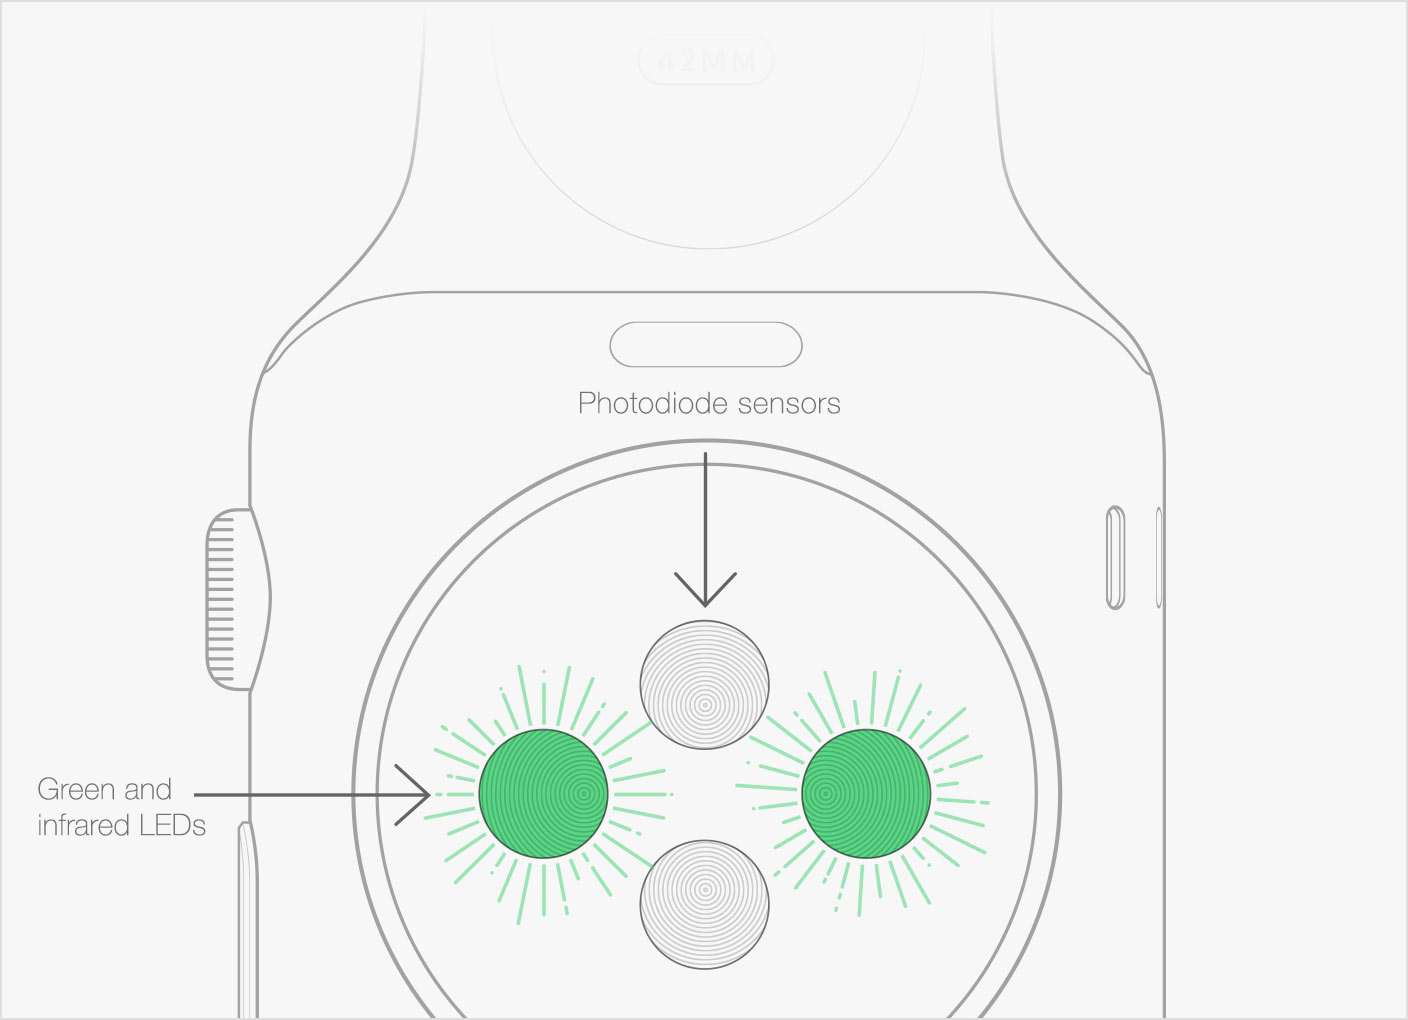
\includegraphics[scale=0.17]{watch-measure-sensors}
	\captionof{figure}{Illustration of the sensor on an Apple Watch}
	\source{\url{https://support.apple.com/en-us/HT204666}}
\end{figure}
%
Fitbit's PurePulse technology is making use of the PPG technique, and so are the Basis Peak HR and the Microsoft Band II.

Many factors effect the performance of the heart rate sensor. 
If the amount of blood flowing through your skin is too low, the heart rate sensor will not get an accurate reading. 
Motion also plays a role: irregular movements decrease the accuracy of the sensor. 
Tattoos can also block the light emitted by the sensor.


\subsection{Heart Rate Variability} \label{section:HRV}
Heart rate variability (HRV) is the variation in the time interval between heartbeats.
It can be measured by measuring the time interval between consecutive heartbeats.
To get a better understanding of this, we take a look at the ECG of a normal sinus rhythm which can be seen in \Cref{fig:ECG}. In this figure, we also see the so-called QRS complex.
In an ECG, the electrical activity of the heart is measured.
The QRS complex is related to the depolarization of the left and right ventricles. 
By some complex processes (that are out of the scope of this thesis), this depolarization eventually causes both ventricles to contract, resulting in a heartbeat. 
By measuring the interval between two consecutive QRS complexes in an ECG, one can determine the HRV.
%
\begin{figure}
	\centering
	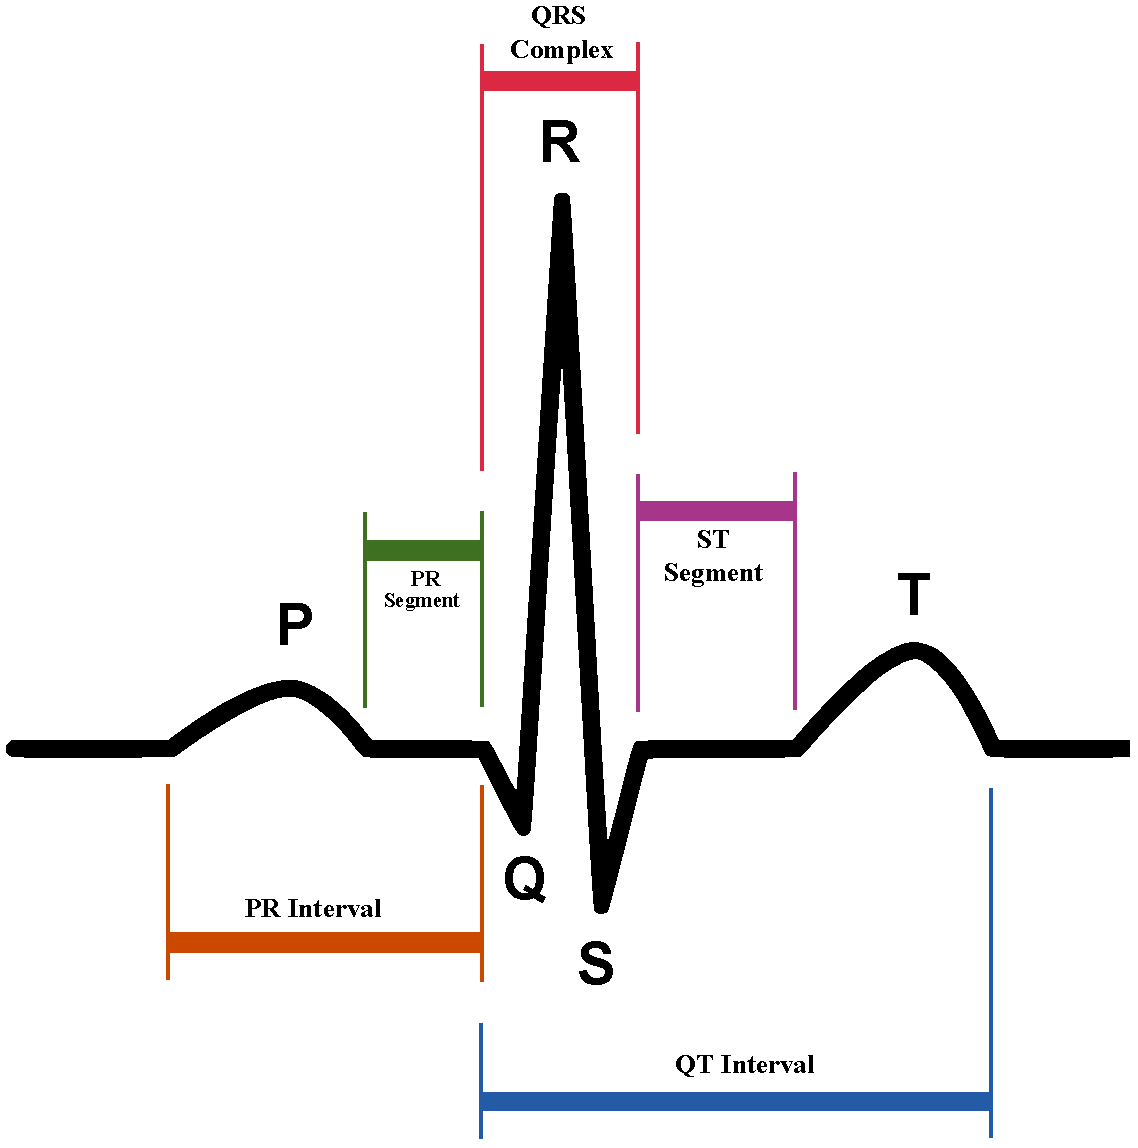
\includegraphics[scale=0.45]{ECG}
	\captionof{figure}{Schematic representation of a normal ECG.}
	\source{Wikipedia}
	\label{fig:ECG}
\end{figure}
%
HRV has proven to be a reliable reflection of the autonomic nervous system, blood pressure and can also be related to gender, sex, age, sleep and diabetes \cite{acharya2006heart}.
The measurements of HRV can generally be grouped under time-domain and frequency domain methods \cite{task1996heart}.
In time domain methods, either the heart rate at any point in time or so called normal-to-normal (NN) intervals between consecutive QRS complexes are determined.
NN is used to make clear that the beats are `normal' beats.
HRV is also referred to as RR variability, where R is the point on the QRS complex.
Some examples of variables that can be calculated when time domain methods are used are the mean heart rate, shortest and longest NN interval and standard deviation.

In frequency domain methods, the heart rate variance is partitioned into underlying rhythms that occur at different frequencies.
Fast Fourier Transform (FFT) is commonly used to find these underlying rhythms.
When this is done, frequencies can be associated with different periodic rhythms.
There are three different rhythms, each with their own frequency range:
%
\begin{itemize}
	\item Very low frequency (VLF) (0.0033 - 0.04 Hz);
	\item Low frequency (LF) (0.04 - 0.15 Hz);
	\item High frequency (HF) (0.15 - 0.4 Hz).
\end{itemize}
%
Afterwards, the NN intervals in each frequency range are counted.

In \cite{thayer2012meta}, HRV as a biomarker for stress was investigated with a meta-analysis of studies.
It was already found that individuals with a greater ability to regulate emotion had greater levels of resting HRV \cite{appelhans2006heart}.

HRV could give more insight in the amount of stress a person is experiencing.
If HRV is a potential biomarker for stress, it must be related to the perception of threat and safety, which are elements of stressors.
That this relation exists was found in \cite{hjortskov2004effect}, where the effect of stress from computer work on HRV and blood pressure was investigated.
Twelve female students participated in the study. They had to perform a computer task where random numbers had to be entered using the keyboard.
The experiment consisted of three stages, in which the participants had to perform the described computer task.
In two of these stages, the experimenter was unfriendly towards his colleagues and unsupportive to the participant. In these stages, the participants also had to perform a memory test.
In the other stage, the experimenter was friendly and supportive, thus eliminating (almost) all stressors.
In this stage no memory test was performed.
Before and after the work, the participants filled in a questionnaire containing a scale to measure the experienced amount of stress.
In stressful situations indicated by the participants, it was found that there was a reduction in the high-frequency component of HRV (calculated from ECG recordings).
An increase in the low- to high-frequency ratio was also found in stressful situations.
The stressors also led to an increase in blood pressure.
This research gives a promising indication for the application of HRV as a biomarker for stress.
In \cite{patel2011applying}, a direct relation was found between the HRV spectrum and fatigue.
In this study, neural network analysis was applied on HRV to assess the fatigue of drivers.
Although the dataset was limited, they managed to get an accuracy of 90\% in predicting whether a given subject was in an alert or in a fatigued state.

\subsection{Two-Minute Walk Test}
During the period of the pilot, MS patients that are participating in our experiment will be asked to do a two-minute walk test (2MWT) every day.
Walking tests are generally used to monitor the effectiveness of a treatment for patients.
The two-minute walk test is a shorter measure of walking performance than the six-minute walk test (6MWT). 
The 2MWT addresses some limitations of the 6MWT.
The latter can be too fatiguing for older people and too time consuming in general.
Especially the limitation of the 6MWT as being too fatiguing, that is addressed in the 2MWT, is relevant for MS patients \cite{gijbels2011comparison}.
Because nerve damage can leave muscles stiff or weak, MS patients can experience a reduced ability to move.
Most of the MS patients also experience fatigue.
Some studies have been done where the measurement properties of the 2MWT were examined \cite{connelly2009clinical} and the reliability and performance was evaluated \cite{bohannon2015two}.
The walking test forces the user to be subjected to physical exertion. 
Therefore, the test can be representative for factors like motivation and fatigue which in turn could be related to day prediction.
In \cite{motl2008worsening}, it was found that a worsening of the symptoms of MS may lead to a reduction of physical activities.
This link could be made visible using the data from the walk test.

As mentioned before, participants will also perform the 2MWT walking test in our experiment.
This will be done using the `Mijn Kwik' app.
This app will record the GPS coordinates as the participants perform the walking test.
The walk test will be initiated as a notification on the phone of the patient.
Only if the GPS accuracy is high enough, the walking test can be started.
This will be explained in more detail in \Cref{section: 2MWT}.

\subsection{Stress} \label{subsection: Stress}
Stress is the response to a stressor. 
A stressor can be an external stimulus or a specific condition in the environment that causes stress.
For humans, stress can be positive or negative. 
Although some forms of stress can have a positive effect on the performance, stress is mostly referred to in a negative way.
Several studies have shown that stress affects MS.
In \cite{buljevac2003self}, researchers investigated the relation of relapsing-remitting MS patients, that experienced attacks, with self-reported stressful events not related to MS.
It was found that the experience of at least one stressful event in a period of four weeks would double the risk of an attack within the next week.
That stress would play an important role in MS has been assumed for a long time.

Some wearables are able to measure the perspiration. 
This is done by measuring  changes in the conductivity of the skin, also called electrodermal activity (EDA), which is related to your sweat production.
The production of sweat is controlled by the sympathetic nervous system.
EDA is related to arousal.
Arousal is the activation state of the autonomic nervous system. 
This is related to the degree of mental awareness or consciousness. 
If the sympathetic nervous system, a branch of the autonomic nervous system, is highly aroused, more sweat will be released resulting in better conductance of the skin.
It will also lead to an increased heart rate and blood pressure.
In addition to motivating certain behaviors like the flight or fight response, arousal also plays an import role in emotion and performance.
Several tasks require different levels of arousals for the best performance.
For example, motivation dependent tasks require higher levels of arousal and concentration dependent tasks require lower levels of arousal for better performance.

In \cite{knufinke2012measurement}, the potential of EDA to measure arousal in a real life setting during exercise was researched. 
This was done using the Affectiva Q\textsuperscript{\texttrademark} sensor that was developed in \cite{poh2010wearable}. This sensor is designed to continuously measure EDA during everyday activities. 
While the measurement of heart rate can also be used to measure levels of arousal, heart rate is influenced by energy demand. Therefore, heart rate is only useful for the measurement of arousal in a resting state, in which energy demand is not influencing the heart rate.
\cite{knufinke2012measurement} illustrated that the measurement of arousal can be done in a high intensive real life setting, which is very promising for daily use of this sensor for MS patients.
%http://www.psychfysio.nl/3_12_2/Arousal is also intertwined with stress.

\subsection{Sitting, Walking and Lying Pattern}
Most of the activity trackers nowadays are able to determine which activity you are doing right now. These activities include walking, running and walking.
We can go into more detail by also keeping track of sitting, walking and lying patterns.

Fatigue is a common symptom for MS patients. 
Researchers have identified the characteristics of so called MS fatigue, that differs from normal fatigue \cite{msfatique}.
These characteristics of fatigue include:
%
\begin{itemize}
	\item Occurring on a daily basis;
	\item Coming easily and suddenly;
	\item Being generally more severe than normal fatigue.
\end{itemize}
%
We could use data from the wearables to get more insight in the pattern of sitting, walking and lying. 
This gives insight in the degree of functional ability and the level of activity during the day.
This could be related to the feeling of a person.
Several studies have researched the classification of activities. 
In \cite{sharma2008frequency}, data from a triaxial accelerometer sensor was used for activity classification.  
The algorithm used for classification was able to classify running, walking and resting activities. 
According to the authors, the algorithm could be extended to also classify activities like standing and sitting.
That this is possible was shown in \cite{karantonis2006implementation}, where a real-time movement classifier was created that could classify activities including falling, sitting, lying (including positions) and standing.
The data being used was collected using a waist-mounted triaxial accelerometer. 
Because the classification was done in real time, the following constraints had to be satisfied:
%
\begin{itemize}
	\item No knowledge of future events;
	\item Amount of buffered data is limited;
	\item Limited processing time: the device must be able to handle the continuous flow of incoming data.
\end{itemize}
% 
When using this data for assessing the quality of upcoming days, the real-time constraints described before are not compulsory.
Data can be send in batches to the database, from which the data can be fetched and used for data mining.
In the described experiment, these real-time constraints led to some limitations of the developed system.
However the experimental results showed that the system was able to classify most activities with a high accuracy.

\subsection{Weather} \label{section:Weather}
That weather can influence your mood is something that many people have experienced. 
That this is no coincidence is confirmed by several studies.
\cite{howarth1984multidimensional} related multiple mood and weather variables.
In this study, it was found that weather was a major predictor for changes in mood. 
For example, a high humidity had a dominant influence on multiple mood variables: 
%
\begin{itemize}
	\item Decrease of concentration and potency;
	\item Increase of sleepiness and fatigue.
\end{itemize}
%
Because some weather data is freely available on the internet, it can be used easily for assessing day quality.
During a meeting with MS patients organized by Orikami, it was found that some patients were more at ease during the summer, while others experienced the same during cold periods.
Heat sensitivity of MS patients is something that has been subjected to extensive research.
In \cite{krupp1988fatigue}, fatigue in MS was investigated. 
This was done by conducting structured interviews with 32 people having MS and 33 healthy adults. 
There were several questions about the characteristics of their fatigue, one of which was ``Heat worsens it". 92\% of the MS patients answered this question with `yes'.
Increased body temperature also seems to influences MS patients. 
In \cite{avis1995sudden}, two cases were described in which heat exposure resulted in death for two patients having MS.
In these cases, exposure to sun (and therefore heat) led to incapacitation of the patients, resulting in death.
Although heat can enlighten the symptoms of MS, it can thus be very dangerous by causing sudden collapses of the thermoregulatory system.

\subsection{Biorhythm}
The theory of biorhythm claims that our life is influenced by rhythmic cycles.
The theory is an example of pseudoscience, which means that it is presented as scientific but does not adhere to the scientific method.
According to the biorhythm theory, three different cycles oscillating in a sine wave (\Cref{fig:biocycles}) influence three different aspects of our life \cite{hines1998comprehensive}. 
The three cycles are:
%
\begin{itemize}
	\item A 23 day cycle that influences \textbf{physical} aspects of behavior. 
	The equation for this cycle is $\sin(2\pi t/23)$.
	
	\item A 28 cycle that influences \textbf{emotions}.
	The equation for this cycle is $\sin(2\pi t/28)$.
	
	\item A 33 day cycle that influences \textbf{intellectual} functions. 
	The equation for this cycle is $\sin(2\pi t/33)$.
\end{itemize}
%
\begin{figure}
	\centering
	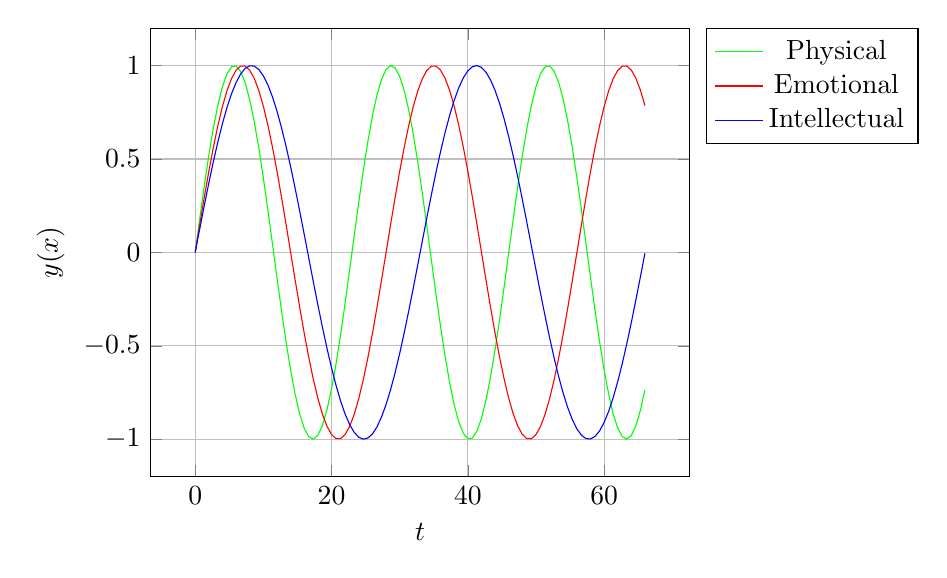
\begin{tikzpicture}
		\begin{axis}[domain=0:21*pi, samples=100,grid=major,
			restrict y to domain=-3:3,xlabel=$t$,ylabel=$y(x)$, legend pos=outer north east]
			\addplot [color=green]    	{sin(deg(x)*2*pi/23};
			\addplot [color=red]  		{sin(deg(x)*2*pi/28};
			\addplot [color=blue] 		{sin(deg(x)*2*pi/33}; 
			\legend{Physical, Emotional, Intellectual}
		\end{axis}
	\end{tikzpicture}
		\captionof{figure}{Biorhythm of the first 66 days after birth.}
		\label{fig:biocycles}
\end{figure}
%
In each of the equations, $t$ indicates the number of days since birth.
According to modern biorhythm theory, these cycles start at the moment of birth and proceed to exist during the rest our lives. 
The durations of these periods do not change.
The required knowledge to apply this theory gives us a great advantage.
By only having knowledge of an individual's date of birth, one is able to calculate the position on each cycle of a particular person, giving insight in the current state for each of the cycles. However, the theory of biorhythm remains controversial.
No scientific evidence has been found that supports the theory.
Some researchers even claim that it has no more predictive power than chance.
It might be worth using biorhythm as a biomarker for day quality, despite its restricted expressive power.

\subsection{Fatigue}
Questionnaires in general can help to retrieve useful information from the user.
The `Mijn Kwik' app, which is also used for the 2MWT experiment, contains questionnaires as well.
The corresponding questions can be seen in \Cref{fig:app} in \Cref{section: Data storage}.
An example of such a question is the slider that can be used by a patient to indicate how energetic he is feeling right now.
Such a question is just one indicator.
There is no simple measure to determine if someone is fatigued, there are just different ways of estimating the level of fatigue.
Below we will discuss several scales that could be used in questionnaires.

\paragraph{Visual Analogue Scales}
Visual Analogue Scales (VAS) can be used as a psychometric response scale in questionnaires. 
It consists of a straight line, where each end of the line contains an extreme statement.
These statements are two opposite claims, for example the statements `no pain' and `the greatest pain I can imagine'. 
In the case where the patient must indicate how he is feeling today (\Cref{fig:app:mood} in \Cref{section: Data storage}), this scale is also used.
A problem with this method is that it is hard to make a distinction between all the possibilities.
The choice made can only be partly explained by the underling property, making it hard to spot measurement errors.
Due to its simplicity, VAS can easily be used.
However, attention must be paid to its role.
It should never be used alone, due to its biases \cite{torrance2001visual}:
%
\begin{itemize}
	\item Context Bias: a VAS score for a state depends on the number of better and worse states that are present at the same time.
	If a state is included with more states that are better, its value is depressed.
	This is in contrast with the effect that occurs when a state is included with more states being worse: its value is enhanced.
	
	\item End-aversion Bias: this bias refers to the reluctance of some respondents to use the extreme values of the scale, or to use the ends when using a continuous scale.
	
\end{itemize}
%

\paragraph{Samn-Perelli Seven Point Fatigue Scale}
The Samn-Perelli Seven Point Fatigue Scale (SPS) is a 7-point scale with scores ranging from 1 (``fully alert, wide awake'') to 7 (``completely exhausted, unable to function effectively'') \cite{samn1982estimating}, which has been validated and is being used widely.

\paragraph{Karolinska Sleepiness Scale}
The Karolinska Sleepiness Scale (KSS) can be used to evaluate sleepiness. 
It has been validated against EEG activity and is also widely used.
KSS is a one-dimensional scale with scores ranging from 1 (``very alert'') to 9 (``very sleepy, great effort to keep awake'').\\

As we can see, there are a lot of verified techniques to get a measurement of fatigue.
Which technique is the best in this setting could be determined by using these scales throughout the pilot and asking feedback from the participants.  


\subsection{Sleep} \label{section:Sleep}
Sleep is a very important stage of the day in our lives. 
While sleeping, our body comes to rest.
For humans (generally for mammals), sleep can be divided in two types: rapid eye movement (REM) and non-rapid eye movement (NREM).
Each of these types have characteristic features.

\paragraph{REM}
During the REM phase in sleep, there is an increased brain activity compared to when being awake.
The muscles in the body are completely relaxed and the eyes make horizontal and vertical movements. Only during this phase of sleep, people are able to dream.
While sleeping, an adult remains on average 15\% of his sleep in REM phase.
Although it is not completely clear what the function of REM sleep is, there are several hypotheses about the functions of REM sleep.
In general, sleep helps to save memories.
Thus, REM might play a role in the processes that make sure that our memories are stored in our memory (memory consolidation), however REM is not a necessary condition for this process.

In \cite{tsoukalas2012origin}, a totally different theory is proposed, which states that REM sleep evolved out of a defensive reflex called toxic immobility. 
This reflex results in total immobilization of an animal, which creates the suggestion that the animal is dead.
This reflex is useful as a last line of defense when the animal is attacked by a predator.
According to this theory, this reflex has similarities with REM sleep.

\paragraph{NREM}
In this stage of sleeping, there is hardly any eye movement.
In contrary to REM, dreaming is rare in this stage of sleeping and there is no relaxation of the muscles. NREM can be divided in three stages \cite{schulz2008rethinking}. While transitioning from the first to the second stage, the movement of the eyes is reduced. In the last stage, it is more common to fall asleep than in the other stages.

As with the theories for REM, there also exist a lot of theories about the function of sleep:
%
\begin{itemize}
	\item Increases the restoration of the body;
	\item Contributes to the processing of memories;
	\item Dreaming, that can occur during some sleep stages, can help processing experiences.
\end{itemize}
%
When researchers want to get insight in the sleep of one or several persons, sleep studies are conducted. 
A common sleep study is polysomnography (PSG), which is also the gold standard for evaluating a person's sleep.
During this sleep study, the following will be measured \cite{polysomnography}:
%
\begin{itemize}
	\item Oxygen in blood;
	\item Eye movement;
	\item Heart rate;
	\item Brain waves;
	\item Activity of muscles;
	\item Lying position;
	\item Amount of air you breathe in and out.
\end{itemize}
%
Most of these measurements cannot be done with simple activity trackers, but they do provide detailed information about a night of sleep.
This information is based on the movements in your sleep.
At the end of the night, these movements are fed into algorithms that calculate sleep scores based on your relative amount of movement during the night. 
Although they can be a good indicator for your amount of sleep during the day, the quality for some other related measurements are not verified.
This is especially the case for complex information like the time you spend in (N)REM during the night, for which it is unknown how these sleeping states are determined.
Often a sleep score is assigned to a night of sleep.
Some activity trackers show how this score is calculated, but it is hard to say how representative this score is. 
Sleep duration however is something that could be useful when looking at good or bad days.

\subsection{Vitamin D}
Vitamin D plays a very interesting role in the risks of relapses for MS patients. 
It is already known that vitamin D is an environmental factor that plays a role in the development of MS.
In \cite{runia2015multiple}, the relation between vitamin D levels and the risk in relapsing-remitting MS of an exacerbation (a synonym for a relapse) was investigated in a longitudinal study with 73 patients having RRMS. 
It was found that higher levels of vitamin D were associated with a decrease in the risk of exacerbations. 
Vitamin D appears to suppress the autoimmune response of T cells attacking the myelin sheaths of the nerve cells and axons.
When vitamin D was given in a high dose to MS patients, the activity of the T cells dropped significantly.
However, some studies suggest that there is an opposite relation between vitamin D and a decreased risk of exacerbation in MS patients: low vitamin D levels are caused by less time spend outside due to increased disabilities for MS patients \cite{van2007vitamin}.
Vitamin D levels can be influenced by sunlight.
The effectiveness of exposing the skin to sunlight, and thereby `getting' vitamin D, depends on several factors:
%
\begin{itemize}
	\item \textbf{Color of the skin}. People with a darker skin tone tend to produce less vitamin D when being exposed to sunlight.
	\item \textbf{Time of the day}. Ultraviolet B rays (UVB) play a role in the natural way of getting vitamin D. 
	When the sun is shining on the earth at a large angle, these UVB rays are blocked. 
	Thus during early and late parts of the day, exposing your skin to the sun will not help in the synthesis of vitamin D.
	\item \textbf{Where you live}. The closer you live to the equator, the easier it will be for your body to synthesize vitamin D from UVB rays. 
\end{itemize}
%
It was already known that vitamin D had a protective effect at the start of MS, but new research shows that it can also effect the course of the disease. 
With the data from wearables, it might be possible to get an approximation of the time spent outdoors.
Because time spent outdoors can influence vitamin D levels, the chance or increased risk of an exacerbation could be determined.

\subsection{Neurogenesis} \label{subsection: Neurogenesis}
Neurogenesis is the name of the process responsible for growing new neurons.
The hippocampus is a place in the brain of the human body where new neurons can be created.
Neurogenesis plays an important role in learning, memory, mood and emotion \cite{smithimpact}.
What is also mentioned in this research, is that there is a clear relation between neurogenesis and depression.
A reduced adult hippocampal neurogenesis (AHN) in different animal models, where antidepressants were able to restore this, is supporting this relation \cite{malberg2003cell, dranovsky2006hippocampal}.
It is also possible to influence the process of neurogenesis. 
In \cite{stangl2009impact}, an overview of different diets, and their influence on AHN for rats and mice was given.
Diets consisting of high saturated fat, were found to reduce the production of new neurons. The same effect was found for the intake of ethanol, that is present in alcohol.
Intermittent fasting and reducing your calorie intake were found to increase neurogenesis.
This effect was also found for foods with a soft texture.

Despite the fact that a lot more factors influence depression and mood, in theory it would be possible to predict levels of depression based on someones diet.
This would make it possible to prevent the effect of stress and even prevent depression.
Because the evidence for the mediation of AHN on the effect of diets on mental health is limited, more studies are needed to confirm this relation. 
In \Cref{table:effectsneurogenesis}, the effect on neurogenesis for some activities or events is given.
%
\begin{table}
	\centering
	\begin{tabular}{@{}ll@{}}
		\toprule
		\multicolumn{2}{l}{\textbf{Effect on neurogenesis}} \\
		\cline{0-1}
		\textbf{Increases} & \textbf{Decrease}  \\ \midrule
		Running & Aging\\
		Sex & Sleep deprivation\\
		Learning & Stress \\ \bottomrule
	\end{tabular}
	\captionof{table}{Events that increase or decrease neurogenesis \cite{thuret2015grow}.}
	\label{table:effectsneurogenesis}
\end{table}
%